%% TC adaptation: compact problem model and requirements.

\begin{figure*}[t]
  \centering
  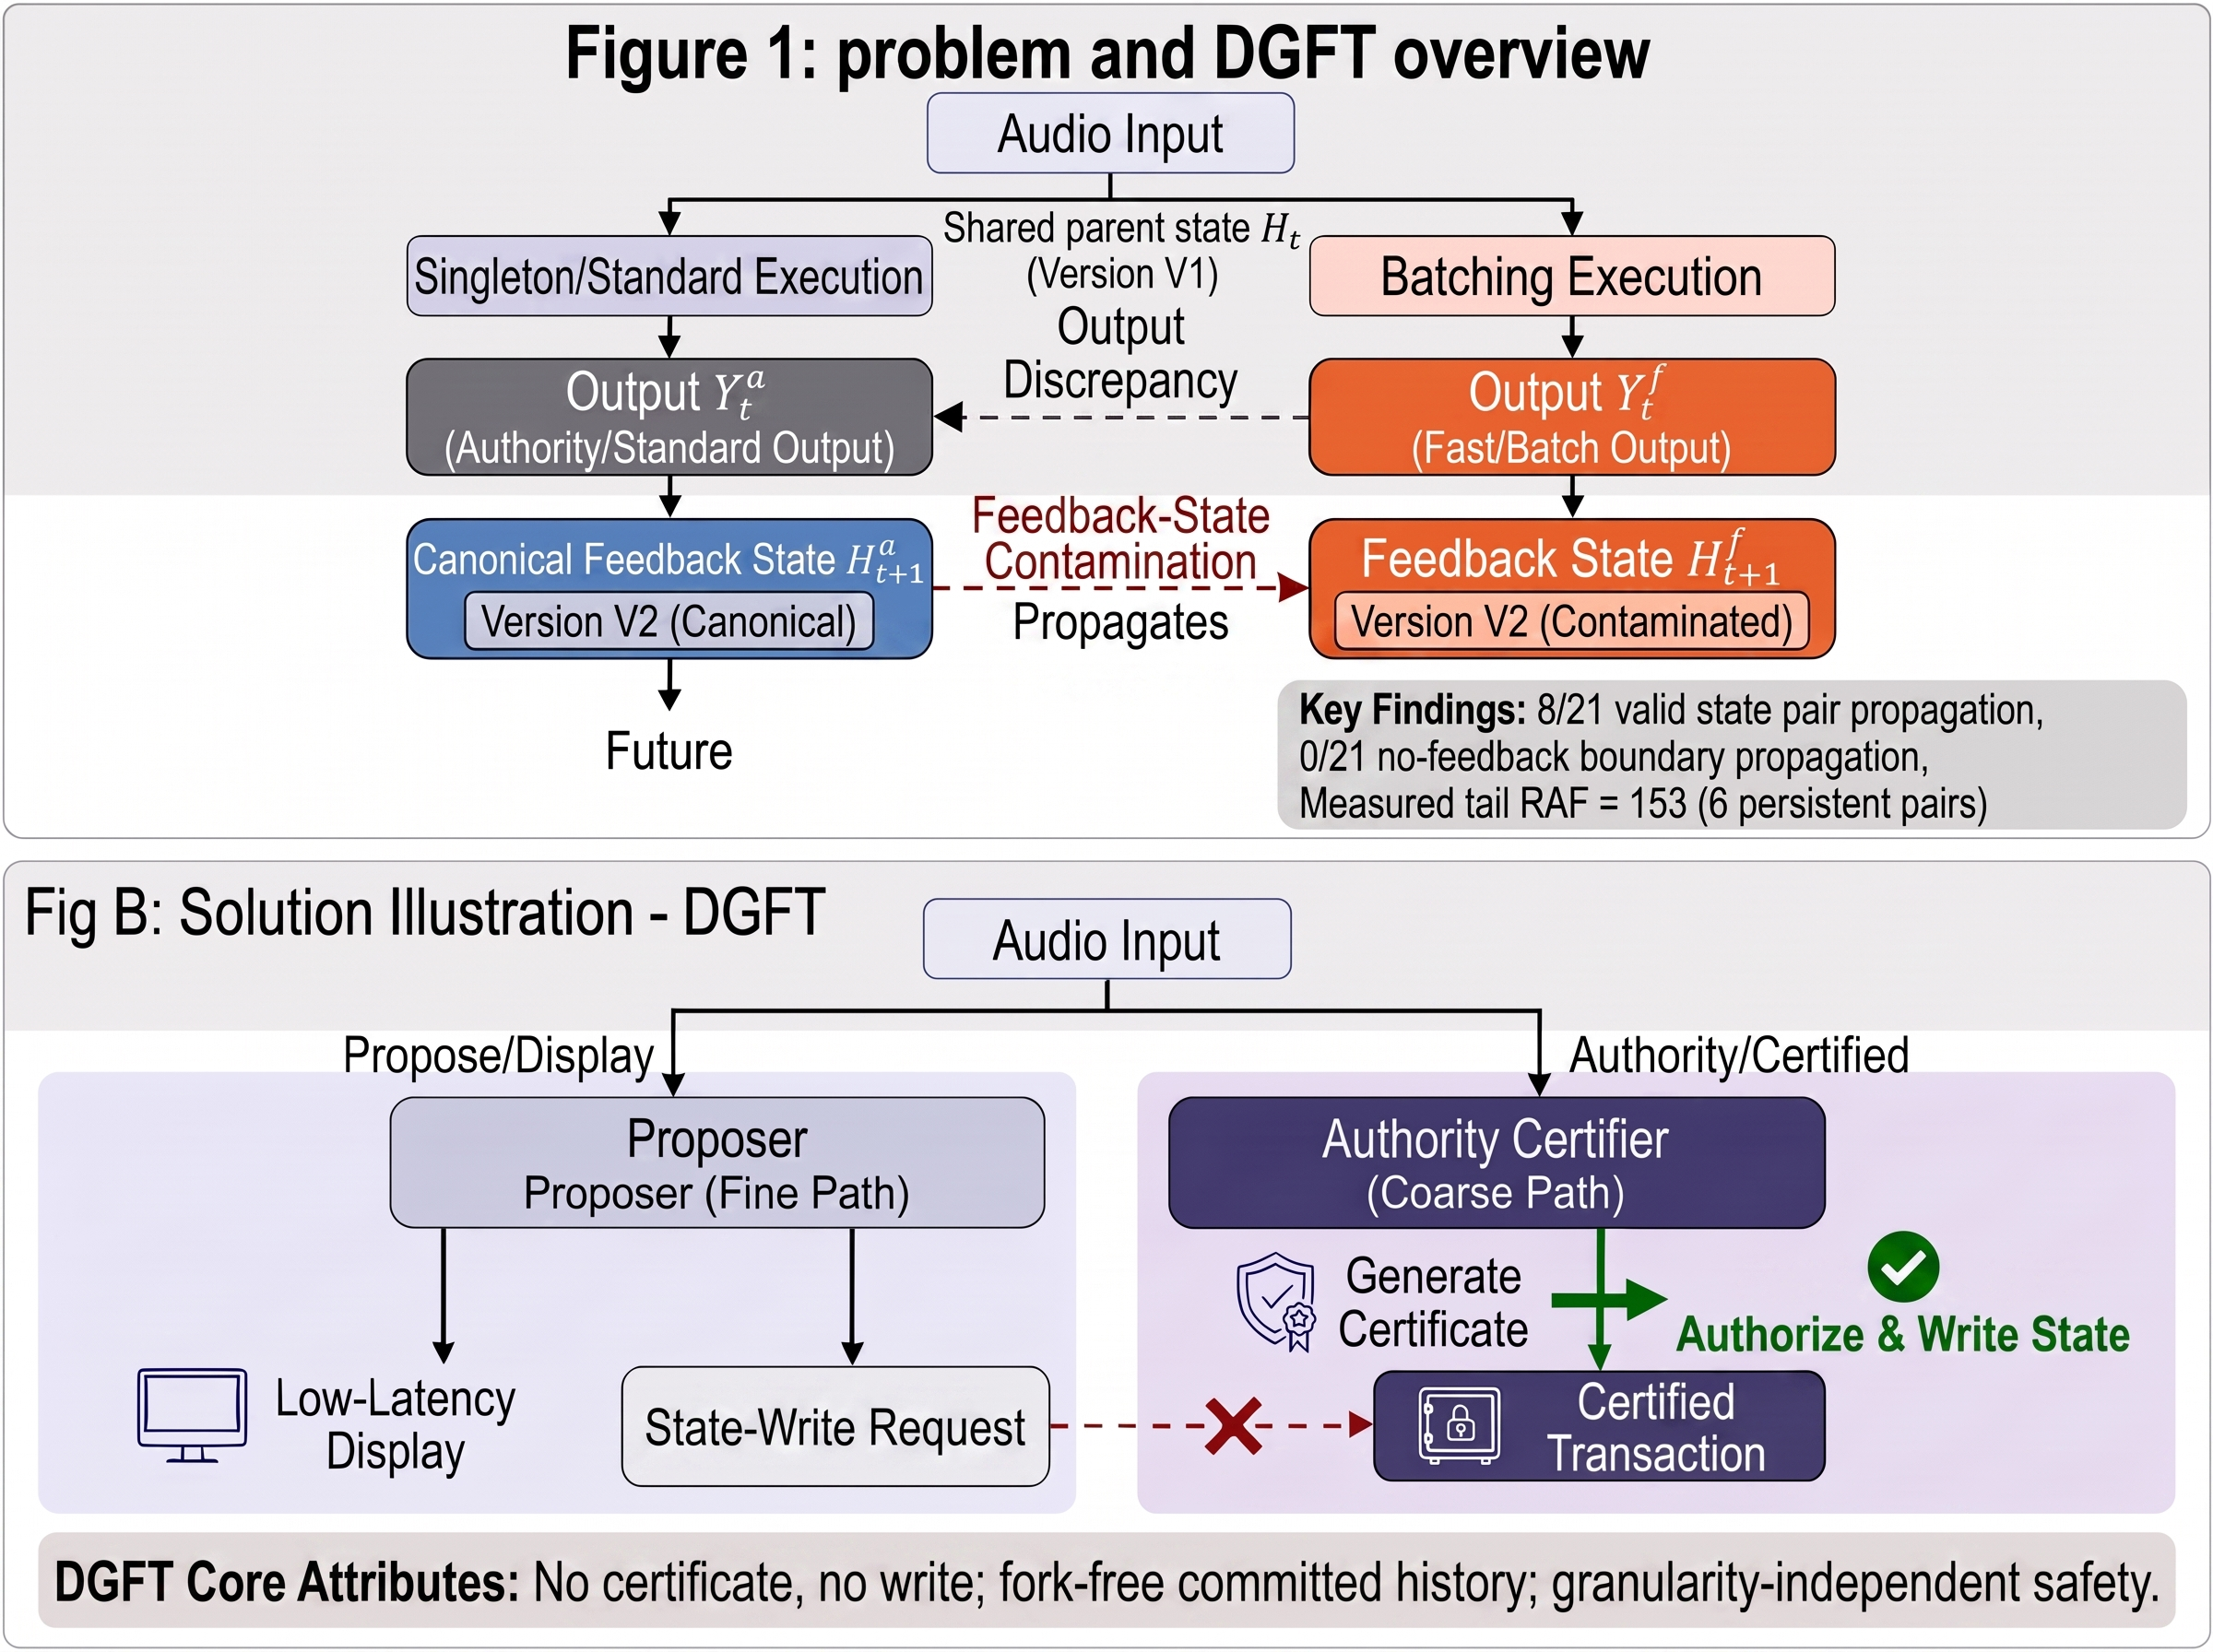
\includegraphics[width=0.96\textwidth]{figures/f1_motivation_senior.jpg}
  \caption{State-entry contamination under ordinary batching (a) and DGFT
  (b). Provisional outputs may differ; only certificate-authorized projections
  may become parents of future state.}
  \label{fig:motivation}
\end{figure*}

\subsection{Revision-generative state machines}\label{sec:model:rsm}

\begin{definition}[Revision-generative serving round]\label{def:rsm}
Round $t$ is $(\state_t,\audio_t,\out_t)$, where $\state_t$ is committed state,
$\audio_t$ is exogenous input (the audio frontier), and $\out_t$ is generated
output. Its update is
\begin{equation}\label{eq:state-update}
  \state_{t+1}=\mathcal{T}(\state_t,\audio_t,\out_t).
\end{equation}
The system is \emph{revision-generative} when $\mathcal{T}$ depends on
$\out_t$, so round $t$ affects state read by round $t{+}1$.
\end{definition}

\begin{definition}[Feedback sub-state and projection]\label{def:projection}
Write $\state_t=(\state_t^x,H_t)$, where $H_t$ is generated feedback and
$\state_t^x$ contains exogenous/runtime conditions held fixed in a causal
pair. The adapter projection $\proj$ writes
\begin{equation}\label{eq:feedback-update}
  H_{t+1}=\proj(\out_t;H_t),
\end{equation}
and the full update factors as
\begin{equation}\label{eq:state-update-h}
  \state_{t+1}=\mathcal{G}(\state_t^x,H_{t+1},\audio_t).
\end{equation}
For Qwen3-ASR, $H_t$ is the rollback prefix~\cite{shi2026qwen3asr}; for
Whisper with previous-text conditioning, it is the prompt~\cite{radford2023whisper}.
\end{definition}

The \emph{feedback edge} is the dependency
$\out_t\rightarrow H_{t+1}$ in Eq.~\eqref{eq:feedback-update}; removing it
makes the next feedback state independent of $\out_t$ while holding future
inputs and runtime assignments fixed. Ordinary batching instead installs
\begin{equation}\label{eq:implicit}
  H_{t+1}=\proj(\out_t^{\mathrm{batch}};H_t),
\end{equation}
without a separate state-write decision.

\subsection{Display output versus state projection}\label{sec:model:display}

Display-only suffixes, hold-back regions, and provisional hypotheses may be
visible while excluded from $\proj$ by the adapter. DGFT therefore enforces
the permission boundary
\begin{equation}\label{eq:invariant}
  \boxed{\mathrm{Display}(\out_t)\;\nRightarrow\;
  \mathrm{Authorize}(\proj(\out_t;H_t)).}
\end{equation}

\subsection{State-entry divergence and contamination}\label{sec:model:divergence}

For the same round, let $\out_t^f$ and $\out_t^a$ denote fine (batched)
proposal and canonical authority outputs.

\begin{definition}[Output divergence]\label{def:eps}
$\varepsilon_t=d_{\out}(\out_t^f,\out_t^a)$, where $d_{\out}$ is the
contract's output-space distance.
\end{definition}

\begin{definition}[State-entry divergence]\label{def:e}
For $P_t^f=\proj(\out_t^f;H_t)$ and
$P_t^a=\proj(\out_t^a;H_t)$,
$\ediv_t=d_{\state}(P_t^f,P_t^a)$ under the same mixed-unit metric.
\end{definition}

\begin{definition}[Contamination event]\label{def:contamination}
\[
  \cont_t \Longleftrightarrow \ediv_t>0\ \wedge\
  \proj(\out_t^f;H_t)\text{ is installed into }H_{t+1}.
\]
Thus output difference alone is not contamination; it must acquire
future-state write permission.
\end{definition}

\subsection{Feedback amplification}\label{sec:model:amplification}

Let $\dist_t=d_H(H_t^f,H_t^a)$ be trajectory distance under identical future
exogenous inputs and assignments.

\begin{assumption}[Local sensitivity]\label{ass:local}
Within the evaluated neighborhood of the canonical trajectory, finite
$L_t,\beta_t$ satisfy
\begin{equation}\label{eq:recurrence}
  \dist_{t+1}\le L_t\dist_t+\beta_t\ediv_t.
\end{equation}
The coefficients are unknown and the assumption makes no global Lipschitz
claim; the decomposition identifies propagation channels only.
\end{assumption}

\begin{remark}[Causal prediction]\label{rem:causal}
Removing the feedback edge sets $\beta_t=0$ for the intervened transition, so
an isolated state-entry perturbation cannot propagate through that edge when
future inputs, assignments, and arithmetic realizations are equal. A fresh
later divergence remains possible. Section~\ref{sec:eval} tests this scoped
prediction.
\end{remark}

\begin{definition}[Revision amplification factor]\label{def:raf}
For horizon $K$,
\[
  \mathrm{RAF}_{t,K}=\frac{\dist_{t+K}}{\ediv_t+\epsilon_0}
\]
is a measured trajectory indicator, not a theoretical bound.
\end{definition}

\subsection{Design requirements}\label{sec:model:reqs}

The model yields four requirements for certified feedback state:
\begin{description}
  \item[R1 (Authority separation).] Display and state-write permissions are
    distinct (Eq.~\eqref{eq:invariant}).
  \item[R2 (Parent ownership).] A projection commits only to the parent
    version against which it was computed.
  \item[R3 (Frontier monotonicity).] Committed audio intervals advance without
    gaps or overlap, forming one history.
  \item[R4 (Evidence non-authority).] Statistical evidence may schedule
    verification but never authorize installation.
\end{description}
Section~\ref{sec:dgft} realizes R1--R4 as protocol checks; Fig.~\ref{fig:arch}
and Table~\ref{tab:guarantees} trace them through the runtime and baselines.
